% !TEX TS-program = XeLaTeX-shellescape
\documentclass[10pt, compress]{beamer}

\usetheme{m}

\usepackage{booktabs}
\usepackage[scale=2]{ccicons}
\usepackage{minted}
\usepackage{tikz}
\usemintedstyle{trac}
\newcounter{mycount}

\tikzset{
	mygrid/.pic={
		  
\draw[step=1cm,color=gray] (-2,-2) grid (3,3);
    \node[fill=cyan] at (-1.5,2.5) {};
    \node[fill=cyan] at (0.5,2.5) {};
    \node[fill=cyan] at (-.5,.5) {};
    \node[fill=cyan] at (2.5,.5) {};
    \node[fill=cyan] at (-1.5,2.5) {};
    \node[fill=cyan] at (1.5,-.5) {};
    \node[fill=cyan] at (-1.5,-1.5) {};

\setcounter{mycount}{1}
\foreach \y in {+2.6,+1.6,.6,-.4,-1.4}
  \foreach \x in {-1.6,-0.6,.4,1.4,2.4}
    \node at (\x,\y)[anchor=north west] {\tiny\arabic{mycount}\addtocounter{mycount}{1}};


	}}



\title{Locating Parks with a Lexicographic Multiobjective Optimization Method}
\subtitle{Under the tutelage of Shahriari}
\date{\today}
\author{Alan Peral}
\institute{Pomona College}


%
% /Library/TeX/texbin:/Users/Boby/miniconda3/bin
%
\begin{document}

\maketitle
\section{Background Info}
\begin{frame}[fragile]
  \frametitle{}

	\begin{block}{What does this mean?}
	\end{block}

\end{frame}

\begin{frame}{Build more parks}

  \begin{itemize}[<+- | alert@+>]
    \item Parks have benefits!
    \item Bogot\'{a}'s master plan
    \item Parks department 
    \item Competing objectives 
   \end{itemize}
\end{frame}

\plain{Essentially}{\vspace{-2em}\begin{center}
\includegraphics[width=14em]{images/leslie-knope.png}\end{center}}



\section{A Basic Example}
\begin{frame}[fragile]
  \frametitle{Example}
  \begin{center}
  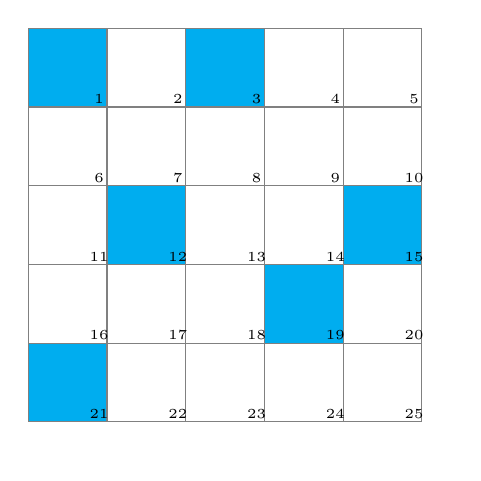
\begin{tikzpicture}[every node/.style={minimum size=1cm-\pgflinewidth}]
  \pic{mygrid};
\end{tikzpicture}
 \end{center}
This is our $5\times5$ grid city

\end{frame}

\begin{frame}[fragile]
  \frametitle{Example}
  \begin{center}
   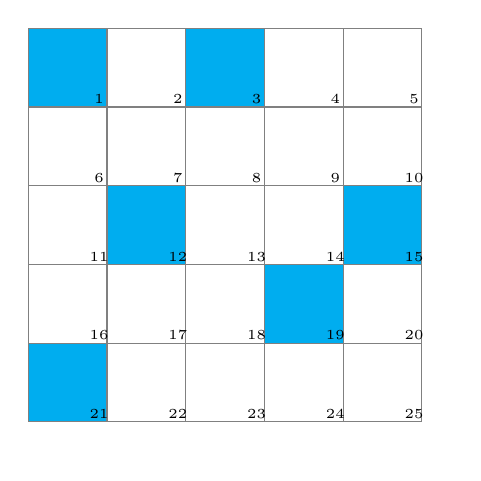
\begin{tikzpicture}[every node/.style={minimum size=1cm-\pgflinewidth}]
  \pic{mygrid};
\end{tikzpicture}
\end{center}
Maybe call it Pawnee.
\end{frame}

\begin{frame}[fragile]
  \frametitle{Example}
  \begin{center}
 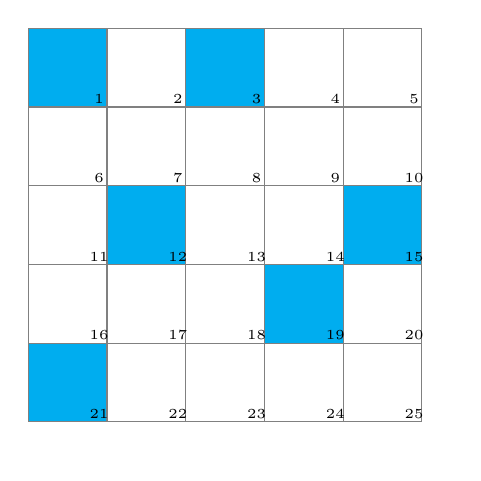
\begin{tikzpicture}[every node/.style={minimum size=1cm-\pgflinewidth}]
  \pic{mygrid};
\end{tikzpicture}
\end{center}
But definitely not.
\end{frame}

\begin{frame}[fragile]
  \frametitle{Example}
  \begin{center}
 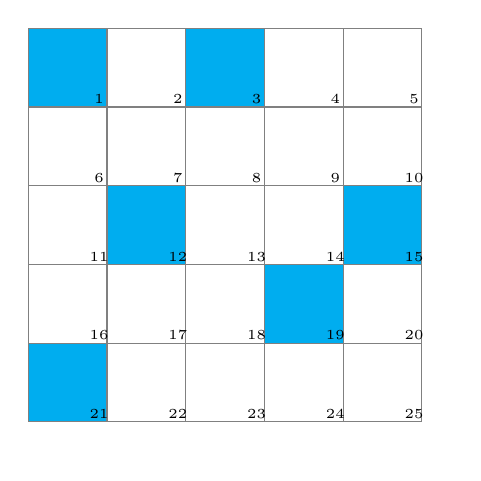
\begin{tikzpicture}[every node/.style={minimum size=1cm-\pgflinewidth}]
  \pic{mygrid};
\end{tikzpicture}
\end{center}
\begin{itemize}
\item Candidate parcels
\end{itemize}
\end{frame}

\begin{frame}[fragile]
  \frametitle{Example}
  \begin{center}
 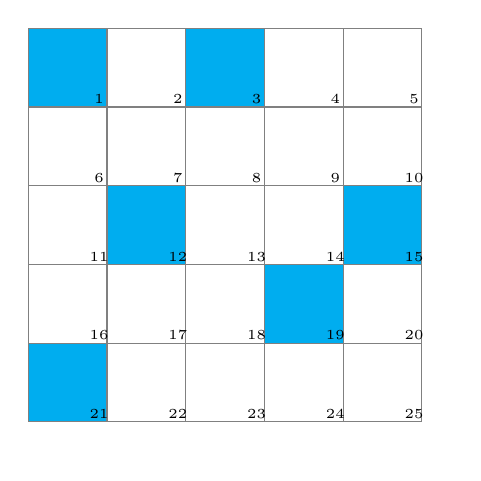
\begin{tikzpicture}[every node/.style={minimum size=1cm-\pgflinewidth}]
  \pic{mygrid};
\end{tikzpicture}
\end{center}
\begin{itemize}
\item Candidate parcels
\item Every lot same size
\end{itemize}
\end{frame}

\begin{frame}[fragile]
  \frametitle{Example}
  \begin{center}
 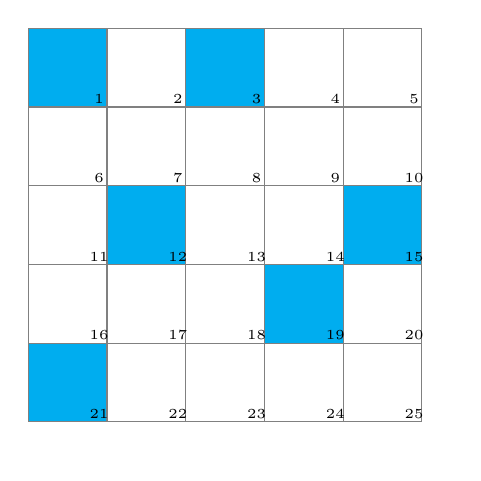
\begin{tikzpicture}[every node/.style={minimum size=1cm-\pgflinewidth}]
  \pic{mygrid};
\end{tikzpicture}
\end{center}
\begin{itemize}
\item Candidate parcels
\item Every lot same size
\item Service area
\end{itemize}
\end{frame}

\begin{frame}[fragile]
  \frametitle{Example}
  \begin{center}
 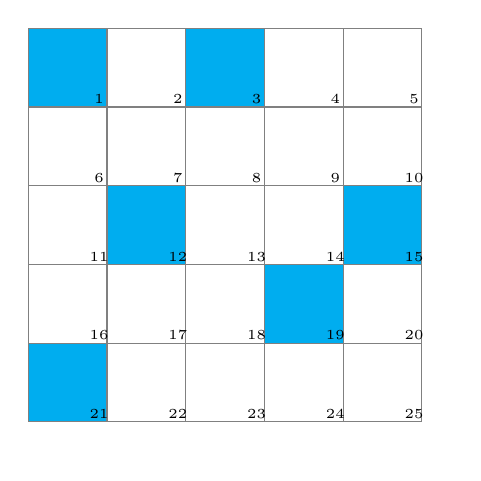
\begin{tikzpicture}[every node/.style={minimum size=1cm-\pgflinewidth}]
  \pic{mygrid};
\end{tikzpicture}
\end{center}
\begin{block}{Which candidate parcel will maximize geographical coverage?}
\end{block}
\end{frame}

\begin{frame}[fragile]
  \frametitle{Example}
  \begin{center}
 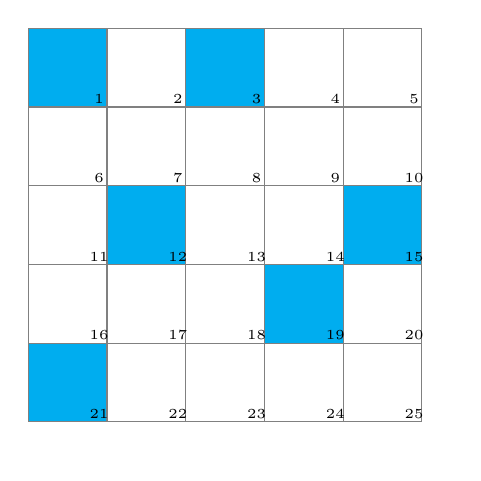
\begin{tikzpicture}[every node/.style={minimum size=1cm-\pgflinewidth}]
  \pic{mygrid};
\end{tikzpicture}
\end{center}
\begin{block}{Which candidate parcel will maximize geographical coverage?}
\alert{Candidate 12}
\end{block}
\end{frame}

\begin{frame}[fragile]
\frametitle{Some Math}
\begin{align*}
\textrm{max } f_1 &= \sum_{j \in \mathcal{J}} z_j \\
\textrm{subject to } z_j &\leq \sum_{i \in \mathcal{W}_j} y_i, j \in \mathcal{J}\\
\left|\mathcal{W}_j\right|z_j &\geq \sum_{i \in \mathcal{W}_j} y_i, j \in \mathcal{J} \\
z_j &\in \{0,1\}, j \in \mathcal{J} \\
y_i &\in \{0,1\}, i \in \mathcal{I}
\end{align*}
\end{frame}

\begin{frame}[fragile]
\frametitle{Some Math}
\begin{align*}
\textrm{max } f_1 &= \sum_{j \in \mathcal{J}} z_j \\
\end{align*}
\begin{itemize}
\item $\mathcal{J}$ is the set of all blocks that could benefit from a new park 
\end{itemize}
\end{frame}

\begin{frame}[fragile]
  \frametitle{Example}
  \begin{center}
 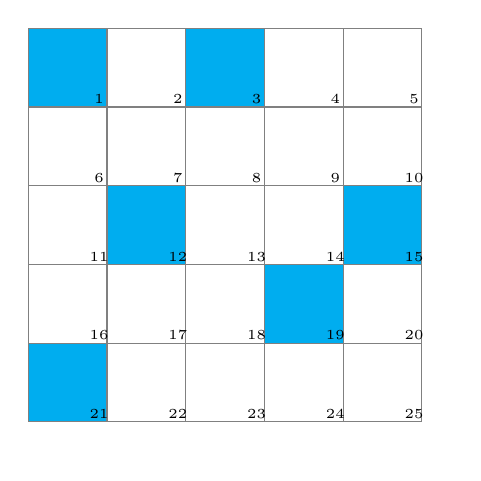
\begin{tikzpicture}[every node/.style={minimum size=1cm-\pgflinewidth}]
  \pic{mygrid};
\end{tikzpicture}
\end{center}
$\mathcal{J} = \{2,4,6,7,8,\dots, 22,23,24,25\}$
\end{frame}

\begin{frame}[fragile]
\frametitle{Some Math}
\begin{align*}
\textrm{max } f_1 &= \sum_{j \in \mathcal{J}} z_j \\
\textrm{subject to } z_j &\in \{0,1\}, j \in \mathcal{J}
\end{align*}
\begin{itemize}
\item $\mathcal{J}$ is the set of all blocks that could benefit from a new park 
\item $z_j$ is a binary decision variable, takes value of 1 if block $j \in \mathcal{J}$ is covered by at least one park, 0 otherwise
\end{itemize}
\end{frame}

\begin{frame}[fragile]
  \frametitle{Example}
  \begin{center}
 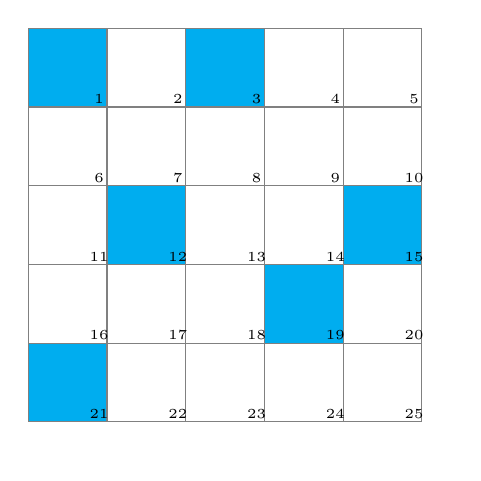
\begin{tikzpicture}[every node/.style={minimum size=1cm-\pgflinewidth}]
  \pic{mygrid};
\end{tikzpicture}
\end{center}
$\mathcal{J} = \{2,4,6,7,8,\dots, 22,23,24,25\}$ \newline
If we chose candidate 21, then $z_7 = 0$ and $z_{16} = z_{17} = z_{22} = 1$ 
\end{frame}

\begin{frame}[fragile]
\frametitle{Some Math}
\begin{align*}
\textrm{max } f_1 &= \sum_{j \in \mathcal{J}} z_j \\
\textrm{subject to } z_j &\leq \sum_{i \in \mathcal{W}_j} y_i, j \in \mathcal{J}\\
z_j &\in \{0,1\}, j \in \mathcal{J} \\
y_i &\in \{0,1\}, i\in \mathcal{I}
\end{align*}
\begin{itemize}
\item $\mathcal{J}$ is the set of all blocks that could benefit from a new park 
\item $z_j$ is a binary decision variable, takes value of 1 if block $j \in \mathcal{J}$ is covered by at least one park, 0 otherwise
\item $\mathcal{I}$ is the set of candidate parcels
\item candidate parcel $i$ belongs to the set $\mathcal{W}_j$ if block $j$ is serviced by parcel $i$
\item $y_i$ a binary decision variable, takes value 1 if candidate $i$ is selected to become a park
\end{itemize}
\end{frame}

\begin{frame}[fragile]
  \frametitle{Example}
  \begin{center}
 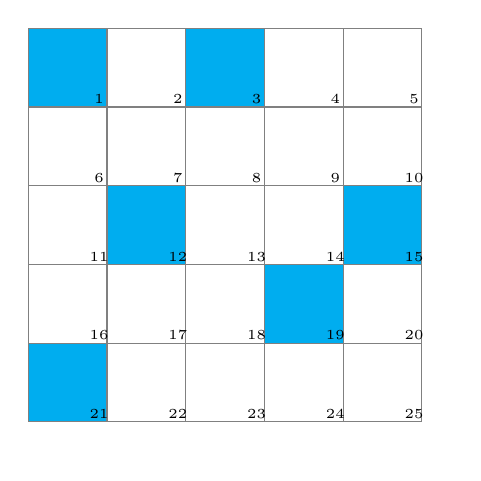
\begin{tikzpicture}[every node/.style={minimum size=1cm-\pgflinewidth}]
  \pic{mygrid};
\end{tikzpicture}
\end{center}
$\mathcal{J} = \{2,4,6,7,8,\dots, 22,23,24,25\}$ \newline
$\mathcal{I} = \{1,3,12,15,19,21\}$
\end{frame}

\begin{frame}[fragile]
  \frametitle{Example}
  \begin{center}
 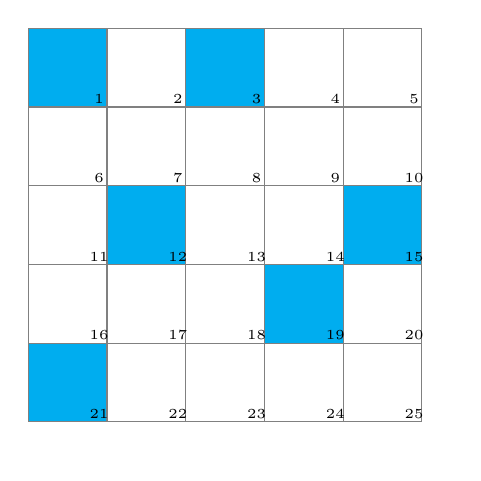
\begin{tikzpicture}[every node/.style={minimum size=1cm-\pgflinewidth}]
  \pic{mygrid};
\end{tikzpicture}
\end{center}
$\mathcal{J} = \{2,4,6,7,8,\dots, 22,23,24,25\}$ \newline
$\mathcal{I} = \{1,3,12,15,19,21\}$ \newline
$\mathcal{W}_7 = \{1,3,12\}$
\end{frame}

\begin{frame}[fragile]
  \frametitle{Example}
  \begin{center}
 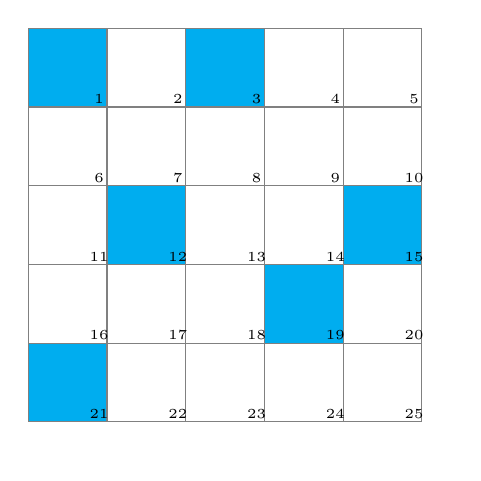
\begin{tikzpicture}[every node/.style={minimum size=1cm-\pgflinewidth}]
  \pic{mygrid};
\end{tikzpicture}
\end{center}
$\mathcal{J} = \{2,4,6,7,8,\dots, 22,23,24,25\}$ \newline
$\mathcal{I} = \{1,3,12,15,19,21\}$ \newline
$\mathcal{W}_7 = \{1,3,12\}$ \newline
If we chose block 21, then $y_{21} = 1$ 
\end{frame}

\begin{frame}[fragile]
\frametitle{Some Math}
\begin{align*}
\textrm{max } f_1 &= \sum_{j \in \mathcal{J}} z_j \\
\textrm{subject to } z_j &\leq \sum_{i \in \mathcal{W}_j} y_i, j \in \mathcal{J}\\
\left|\mathcal{W}_j\right|z_j &\geq \sum_{i \in \mathcal{W}_j} y_i, j \in \mathcal{J} \\
z_j &\in \{0,1\}, j \in \mathcal{J} \\
y_i &\in \{0,1\}, i \in \mathcal{I}
\end{align*}
\begin{itemize}
\item Guarantees that if block $j$ is covered, then at least one candidate parcel covering it has been selected as a park
\item If block $j$ is not covered, then none of the candidate parcels serving it should be selected
\end{itemize}
\end{frame}

\begin{frame}[fragile]
  \frametitle{Example}
  \begin{center}
 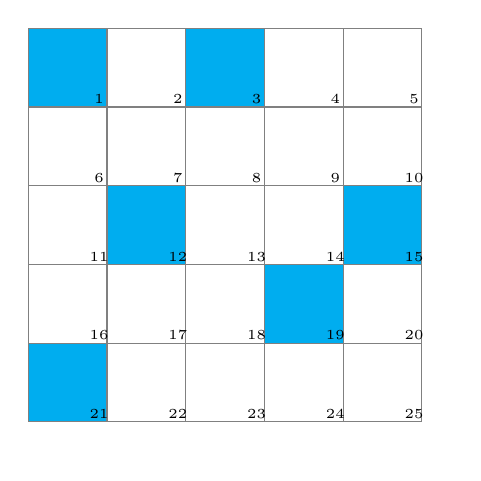
\begin{tikzpicture}[every node/.style={minimum size=1cm-\pgflinewidth}]
  \pic{mygrid};
\end{tikzpicture}
\end{center}
If we chose block 21, then the first constraint becomes \newline
\begin{align*}
z_{16} \leq \sum_{i \in \mathcal{W}_{16}} y_i 
\Rightarrow z_{16} \leq y_{12} + y_{21}
\Rightarrow 1 \leq 0 + 1 
\end{align*}
\end{frame}

\begin{frame}[fragile]
  \frametitle{Example}
  \begin{center}
 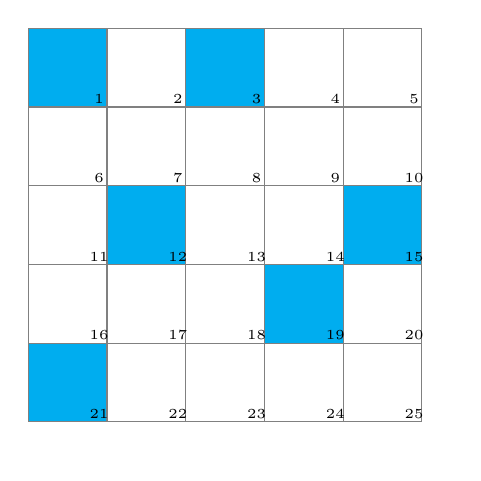
\begin{tikzpicture}[every node/.style={minimum size=1cm-\pgflinewidth}]
  \pic{mygrid};
\end{tikzpicture}
\end{center}
If we chose block 21, then the second constraint becomes \newline
\begin{align*}
\left|\mathcal{W}_4\right|z_4&\geq \sum_{i \in \mathcal{W}_4} y_i 
\Rightarrow (1 \times 0) \geq y_3 
\Rightarrow 0 \geq 0
\end{align*}
\end{frame}

\section{Complications}

\begin{frame}[fragile]
\frametitle{Multiobjective}
\begin{itemize}
\item Maximize number of beneficiaries?
\end{itemize}
\end{frame}

\begin{frame}[fragile]
\frametitle{Multiobjective}
\begin{itemize}
\item Maximize number of beneficiaries?
\item Maximize accessibility?
\end{itemize}
\end{frame}

\begin{frame}[fragile]
\frametitle{Multiobjective}
\begin{itemize}
\item Maximize number of beneficiaries?
\item Maximize accessibility?
\item Maximize connectivity to existing facilities?
\end{itemize}
\end{frame}

\begin{frame}[fragile]
\frametitle{Multiobjective}
\begin{itemize}
\item Maximize number of beneficiaries?
\item Maximize accessibility?
\item Maximize connectivity to existing facilities?
\item Place parks closer to positive facilities (like schools) and further from negative facilities (like waste treatment plants)?
\end{itemize}
\end{frame}


\begin{frame}[fragile]
\frametitle{Multiobjective}
\begin{itemize}
\item Maximize number of beneficiaries?
\item Maximize accessibility?
\item Maximize connectivity to existing facilities?
\item Place parks closer to positive facilities (like schools) and further from negative facilities (like waste treatment plants)?
\item Minimize cost?
\end{itemize}
\end{frame}

\begin{frame}[fragile]
\frametitle{Multiobjective}
\begin{block}{What if we want to do all these things?}
\end{block}
\end{frame}

\begin{frame}[fragile]
\frametitle{Multiobjective}
\begin{block}{What if we want to do all these things?}
Need a way to maximize or minimize multiple objective functions at a time.
\end{block}
\end{frame}

\begin{frame}[fragile]
\frametitle{More Issues}
\begin{itemize}
\item Now what if we had 100 blocks? 1000 blocks? More?
\end{itemize}
\end{frame}

\begin{frame}[fragile]
\frametitle{More Issues}
\begin{itemize}
\item Now what if we had 100 blocks? 1000 blocks? More?
\item What if the parcels weren't all the same size?
\end{itemize}
\end{frame}

\begin{frame}[fragile]
\frametitle{More Issues}
\begin{itemize}
\item Now what if we had 100 blocks? 1000 blocks? More?
\item What if the parcels weren't all the same size?
\item What if the parcels weren't all the same shape?
\end{itemize}
\end{frame}

\begin{frame}[fragile]
\frametitle{More Issues}
\begin{itemize}
\item Now what if we had 100 blocks? 1000 blocks? More?
\item What if the parcels weren't all the same size?
\item What if the parcels weren't all the same shape?
\item How do you measure these things?
\end{itemize}
\end{frame}


\section{Conclusion}

\begin{frame}{Summary}

  Locating parks is a complicated problem.

\end{frame}

\plain{}{Questions?}

\plain{}{\vspace{-2em}\begin{center}
\includegraphics[width=14em]{images/tom-haverford.jpg}\end{center}}



\end{document}